\documentclass[10pt,a4paper]{article}
\usepackage[utf8]{inputenc}
\usepackage[spanish]{babel}
\usepackage{amsmath}
\usepackage{amsfonts}
\usepackage{amssymb}
\usepackage[T1]{fontenc} 
\usepackage[left=2.00cm, right=2.00cm, top=2.00cm, bottom=2.00cm]{geometry}
\usepackage{acronym}
\usepackage{listings}
\usepackage{graphicx}
\graphicspath{ {images/} }
\usepackage{hyperref}

\usepackage{multirow}
\usepackage[table,xcdraw]{xcolor}

\usepackage[export]{adjustbox}
\usepackage{subcaption}

\usepackage[ruled]{algorithm2e}

%%Sobre el código
\usepackage{xcolor}
\usepackage{xparse}
\NewDocumentCommand{\codeword}{v}{%
	\texttt{\textcolor{blue}{#1}}%
}

\setlength{\parindent}{1em}
\setlength{\parskip}{1em}




\title{
Práctica 1\\
\large Aprendizaje Automático \\
}

\author{
Alejandro Palencia Blanco\\
}

\date{05/04/2021}



\begin{document}

\maketitle

\newpage

\tableofcontents

\newpage

\section{Ejercicio sobre la búsqueda iterativa de óptimos}

En este primer ejercicio trabajaremos con el algoritmo de gradietne descendente. Primero, implementaremos el algoritmo y, a continuación, lo ejecutaremos sobre una función $E$ a la que previamente le habremos calculado su gradiente. Después, lo aplicaremos a otra función $f$ con distintas tasas de aprendizaje y puntos iniciales para analizar cómo estos hiperparámetros pueden afectar al mínimo encontrado. Finalmente, llegaremos a una conclusión sobre la dificultad de encontrar el mínimo global de una función arbitraria.



\subsection{Implementación del algoritmo de gradiente descendente}

Gradiente descendente es un algoritmo iterativo que tiene como objetivo encontrar un mínimo local para una función dada. Al iniciar el algoritmo, dicho mínimo toma el valor de un punto inicial $w_0$ previamente elegido y, en cada iteración modifica su valor haciendo uso del gradiente de la función a minimizar y del un hiperparámetro llamado \textit{learning rate}, que marca su velocidad de cambio.

El algoritmo finaliza cuando se supera un número máximo de iteraciones o cuando el error cometido por el mínimo actual es menor que un umbral, lo que ocurra antes. Cabe destacar que el segundo criterio que usa un umbral solo es posible usarlo cuando se tiene cierta información sobre el valor mínimo global de la función (por ejemplo, si la función es no negativa, sabemos que el valor mínimo global no será inferior a 0). Cuando se cumple el criterio de parada, el algoritmo devuelve el mínimo encontrado en la última iteración junto con el número de iteraciones empleadas.

Los parámetros que usa mi implementación son:

\begin{itemize}
	\item $E$: función a minimizar
	\item $gradE$: gradiente de la función a minimizar
	\item $w_0$: punto inicial con el que se empieza a buscar el mínimo
	\item $lr$: tasa de aprendizaje o \textit{learning rate}
	\item $error$: umbral usado en el criterio de parada
	\item $max\_iter$: número máximo de iteraciones usado en el criterio de parada
\end{itemize}


\begin{algorithm}[H]
	\KwData{$E$, $gradE$, $w_0$, $lr$, $error$, $max\_iter$}
	\KwResult{$w$, $iterations$}
	\Begin{
		$w \leftarrow w_0$
		
		$iterations \leftarrow 0$
		
		\While{ $E(w[0],w[1]) \geq error \ and \ iterations < max\_iter$ }{
			$w \leftarrow w - lr*gradE(w[0],w[1])$
			
			$iterations \leftarrow iterations + 1$
		}
	}
	\caption{Gradient Descent}
\end{algorithm}



\subsection{Ejecución del algoritmo de gradiente descendente para la función $E$}

Consideramos la funcion $E(u,v) = (u^3 e^{v-2}-2 v^2 e^{-u})^2$, la cual es diferenciable y podemos calcularle sus derivadas parciales:

\begin{itemize}
	\item $\frac{\partial E}{\partial u}(u,v) = 2(u^3 e^{v-2}-2 v^2 e^{-u}) (3 u^2 e^{v-2} + 2 v^2 e^{-u})$
	\item $\frac{\partial E}{\partial v}(u,v) = 2 (u^3 e^{v-2} - 2 v^2 e^{-u}) (u^3 e^{v-2} - 4 v e^{-u})$
\end{itemize}

Por tanto, el gradiente de $E$ es $$\nabla E(u,v) = (\frac{\partial E}{\partial u},\frac{\partial E}{\partial v})(u,v) = (2(u^3 e^{v-2}-2 v^2 e^{-u}) (3 u^2 e^{v-2} + 2 v^2 e^{-u}), 2 (u^3 e^{v-2} - 2 v^2 e^{-u}) (u^3 e^{v-2} - 4 v e^{-u}))$$

Aplicamos gradiente descendente para hallar un mínimo de esta función. Como $E(u,v) \geq 0 \ \forall (u,v) \in \mathbb{R}^2$ por ser una expresión elevada al cuadrado, entonces sabemos que el mínimo que encontremos no será inferior a 0. Por tanto, tiene sentido usar una condición de parada que utilice un umbral positivo muy cercano a 0. También fijaremos un número máximo de iteraciones para asegurar que el algoritmo para en el caso de que no se encuentre un mínimo por debajo del umbral. Los valores que daremos a estos hiperparámetros serán $error = 10^{-14}$ y $max\_iter = 10^{10}$, respectivamente. La tasa de aprendizaje la fijaremos a $\eta = 0.1$ y tomaremos $w_0 = (1,1)$ como punto inicial.

Tras ejecutar el algoritmo, vemos que este realiza 10 iteraciones antes de parar y devolver un valor de $E$ inferior a $10^{-14}$. El mínimo obtenido es $w = (1.1572888496465497, 0.9108383657484799)$, luego estas fueron las coordenadas en las que se alcanzó por primera vez un valor menor que el error fijado. En la Figura \ref{fig:ej1.2} podemos ver la gráfica de la función $E(u,v)$ junto con el mínimo encontrado por gradiente descendente.

\begin{figure}[h]
	\centering
	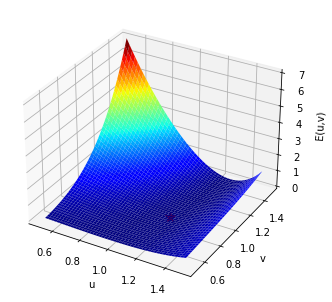
\includegraphics[width=0.6\textwidth]{ej1.2}
	\caption{Gráfica de $E(u,v)$ junto con el mínimo encontrado por gradiente descendente}
	\label{fig:ej1.2}
\end{figure}



\subsection{Ejecución del algoritmo de gradiente descendente para la función $f$}

Consideramos ahora la funcion $f(x,y) = (x+2)^2 + 2 (y-2)^2 + 2 \sin (2 \pi x) \sin (2 \pi y)$, la cual de nuevo es diferenciable y podemos calcularle sus derivadas parciales:

\begin{itemize}
	\item $\frac{\partial f}{\partial x}(u,v) = 2 (x+2) + 4 \pi \cos (2 \pi x) \sin (2 \pi y)$
	\item $\frac{\partial f}{\partial y}(u,v) = 4 (y-2) + 4 \pi \sin (2 \pi x) \cos (2 \pi y)$
\end{itemize}

Por tanto, el gradiente de $f$ es $$\nabla f(x,y) = (\frac{\partial f}{\partial x},\frac{\partial f}{\partial y})(x,y) = (2 (x+2) + 4 \pi \cos (2 \pi x) \sin (2 \pi y), 4 (y-2) + 4 \pi \sin (2 \pi x) \cos (2 \pi y))$$

Esta vez, aplicaremos gradiente descendente con tasas de aprendizaje $\eta = 0.01$ y $\eta = 0.1$ para analizar el impacto que supone tomar distintos valores de $\eta$ en el cálculo del mínimo. Queremos que en ambas ejecuciones se realicen exactamente 50 iteraciones, luego no nos interesa usar el criterio de parada del umbral. Para ello, fijamos $max\_iter = 50$ y $error = -2$, pues se puede ver que $f$ no puede tomar valores inferiores a -2. El punto inicial lo fijamos a $w_0 = (-1, 1)$.

En la Figura \ref{fig:ej1.3_graficas} podemos ver las gráficas de $f$ junto con los mínimos obtenidos para cada una de las tasas de aprendizaje. Para $\eta = 0.01$ obtenemos el mínimo $(-1.269064351751895, 1.2867208738332965)$, mientras que para $\eta = 0.1$ llegamos al mínimo $(-2.939376479816701, 1.607795422435394)$. Como se puede apreciar en ambas, la función $f$ tiene un gran número de mínimos locales que pueden dificultar al gradiente descendente llegar al mínimo global. Analizaremos esto con mayor detenimiento en el siguiente apartado.

\begin{figure}[h]
	\begin{subfigure}{0.5\textwidth}
		\centering
		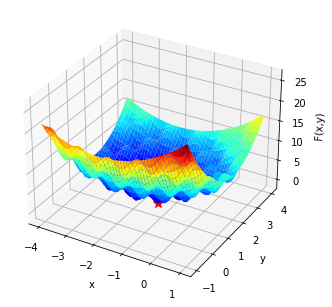
\includegraphics[width=\textwidth]{ej1.3_grafica_eta0.01}
		\caption{$\eta = 0.01$}
	\end{subfigure}
	\begin{subfigure}{0.5\textwidth}
		\centering
		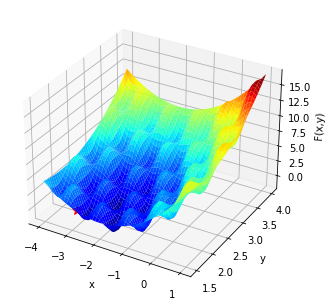
\includegraphics[width=\textwidth]{ej1.3_grafica_eta0.1}
		\caption{$\eta = 0.1$}
	\end{subfigure}
	\caption{Gráfica de $f(x,y)$ junto con el mínimo encontrado por gradiente descendente}
	\label{fig:ej1.3_graficas}
\end{figure}

Por otro lado, si guardamos los valores que nos devuelve la función $f$ para cada uno de los mínimos $w$ obtenidos en cada iteración, podemos generar gráficas que muestren la evolución de dichos valores para ambas tasas de aprendizaje. En la Figura \ref{fig:ej1.3_evolucion} podemos ver esta evolución para $\eta = 0.01$ y $\eta = 0.1$, respectivamente. 

\begin{figure}[h]
	\begin{subfigure}{0.5\textwidth}
		\centering
		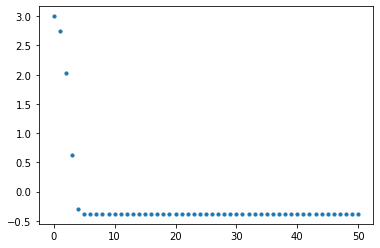
\includegraphics[width=\textwidth]{ej1.3_evolucion_eta0.01}
		\caption{$\eta = 0.01$}
	\end{subfigure}
	\begin{subfigure}{0.5\textwidth}
		\centering
		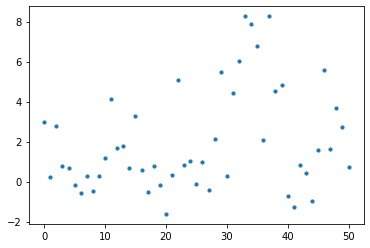
\includegraphics[width=\textwidth]{ej1.3_evolucion_eta0.1}
		\caption{$\eta = 0.1$}
	\end{subfigure}
	\caption{Evolución de los valores devueltos por los mínimos obtenidos en cada iteración}
	\label{fig:ej1.3_evolucion}
\end{figure}

Comprobamos que la evolución obtenida para $\eta = 0.01$ es decreciente, llegando a tener cambios despreciables a partir de la quinta iteración. Sin embargo, para $\eta = 0.1$, la evolución es absolutamente caótica, llegando incluso a empeorar el valor devuelto por el punto de inicio en varias iteraciones. Por tanto, podemos concluir que la elección del valor asignado a la tasa de aprendizaje tiene un gran impacto tanto en el mínimo que obtiene gradiente descendente como en el número de iteraciones necesarias para llegar hasta él. Si el valor de $\eta$ es demasiado grande (en nuestro caso, $\eta = 0.1$), la convergencia hacia un mínimo se vuelve más difícil hasta el punto de que se puede incluso llegar a divergir. Por otro lado, si $\eta$ es demasiado pequeño, el número de iteraciones necesarias para llegar al mínimo puede ser demasiado alto. Lo ideal es que no sea ni demasiado grande ni demasiado pequeño (en nuestro caso, $\eta = 0.01$), para que llegue a converger a un mínimo con una velocidad adecuada.

A continuación, realizaremos otro experimento para analizar la dependencia del mínimo con respecto al punto inicial. Usamos el mismo criterio de parada que antes (50 iteraciones) y fijamos una tasa de aprendizaje $\eta = 0.01$, pues ya hemos visto anteriormente que garantiza que los sucesivos mínimos evolucionen a una velocidd adecuada. Con estos hiperparámetros, tomamos un conjunto de puntos iniciales y ejecutamos gradiente descendente con cada uno de ellos. En el Cuadro \ref{fig:ej1.3_puntos_iniciales} podemos ver los resultados obtenidos.

\begin{table}[]
	\centering
	\begin{tabular}{|r|r|r|}
		\hline
		\multicolumn{1}{|c|}{\textbf{Punto inicial}} & \multicolumn{1}{c|}{\textbf{Mínimo}} & \multicolumn{1}{c|}{\textbf{Valor mínimo}}                          \\ \hline
		(-0.5, -0.5)                                 & (-0.79349947, -0.12596576)           & 9.125146662901855                                                   \\ \hline
		(1.5, 1.5)                                   & (1.16560878, 1.76388342)             & 8.413775701290414                                                   \\ \hline
		(2.1, -2.1)                                  & (0.14880583, -0.0960677)             & 12.490971442685037                                                  \\ \hline
		(-3.0, 3.0)                                  & (-2.73093565, 2.71327913)            & -0.38124949743809955                                                \\ \hline
		(-2.0, 2.0)                                  & (-2.0, 2.0)                          & $-4.799231304517944 \cdot 10^{-31}$                                 \\ \hline
	\end{tabular}
	\caption{Tabla con los mínimos obtenidos para cada punto inicial}
	\label{fig:ej1.3_puntos_iniciales}
\end{table}

Comprobamos que para cada punto inicial obtenemos un mínimo distinto al resto. Además, los valores mínimos que nos devuelven son también muy distintos, pues los tres primeros son mayores que 8 mientras que los dos últimos son inferiores a 0. Esto demuestra que la dependencia con respecto al punto inicial puede llegar a ser muy alta, sobre todo en funciones como ésta que tienen muchos mínimos locales.



\subsection{Conclusión sobre la dificultad de encontrar el mínimo global de una función arbitraria}

El apartado anterior pone de manifiesto la dependencia que puede llegar a tener el mínimo encontrado de hiperparámetros como la tasa de aprendizaje o el punto inicial. Si la función posee un único mínimo (por  ejemplo, si la función es convexa), esta dependencia puede ser mucho menor. Sin embargo, el número de mínimos locales que puede llegar a tener una función arbitraria puede ser infinito, luego la probabilidad de que una ejecución de gradiente descendente acabe atrapada en alguno de estos mínimos puede ser muy alta. La función $f$ del apartado anterior es un ejemplo que ilustra a la perfección este fenómeno. Por tanto, concluimos que para una función arbitraria de la que a priori no conocemos ninguna propiedad que podamos usar a nuestro favor, la dificultad de encontrar su mínimo global es enorme.







\newpage

\section{Ejercicio sobre regresión lineal}

\subsection{Ajuste de modelos de regresión lineal a vectores de características extraídos de imágenes de dígitos manuscritos}

Partimos de un conjunto de datos cuyos vectores de características han sido extraídos de imágenes de dígitos manuscritos. Estas características son dos: intensidad promedio (valor medio del nivel de gris) y simetría con respecto al eje vertical. Además, como para este problema solamente se han seleccionado imágenes dos dígitos diferentes, el 1 y el 5, solo tendremos dos etiquetas (la etiqueta -1 representa al 1 y la etiqueta -1, al 5). A pesar de que éste sea un problema de clasificación, en lugar de elegir un algoritmo de clasificación lineal como perceptrón para resolverlo, haremos uso de dos algoritmos de regresión lineal: gradiente descendente estocástico (SGD) y pseudoinversa.

Para encontrar una solución a nuestro problema, ambos algoritmos utilizan el criterio de minimización del riesgo empírico (ERM). Para ello, se define una función $E_{in}(w)$ llamada error muestral que se busca minimizar para llegar a una solución. Tomando el error cuadrático medio, $E_{in}(w) = \frac{1}{N} \sum_{i=1}^N (x_i w - y_i)^2 = \frac{1}{N} \|Xw-y\|^2$, el teorema de Gauss-Markov nos asegura que una solución que se acerque a un mínimo de $E_{in}$ también será cercana a un mínimo de $E_{out}$, siendo esta última función el error a nivel de población. Esta minimización se lleva a cabo usando el gradiente del error muestral, $\nabla E_{in}(w) = \frac{2}{N} X^T (Xw-y)$.

SGD es similar a gradiente descendente, pero con la diferencia de que el conjunto de datos se particiona aleatoriamente en minibatches y, en cada iteración, en lugar de usar el conjunto de datos completo, usamos un único minibatch para actualizar los pesos. Cuando hemos agotado todos los minibatches, volvemos a particionar aleatoriamente el conjunto de datos y continuamos actualizando los pesos con los nuevos minibatches. Cada uno de estos periodos desde que se extraen nuevos minibatches hasta que todos ellos han sido usados se denomina época. Este algoritmo añade una componente estocástica a gradiente descendente que proporciona una mayor variabilidad en la estimación del gradiente, además de ser más rápido en el cómputo del mismo.

Por otro lado, el algoritmo de la pseudoinversa intenta resolver el problema en un único paso calculando la matriz pseudoinversa de $X$, $X^{\dag} = (X^T X)^{-1} X^T$. A partir de ella, podemos tomar $w = X^{\dag} y$, solución que garantiza que $\nabla E_{in}(w) = 0$.

Para resolver este apartado, he definido la función de pérdida \codeword{Err}, que calcula el error cuadrático medio, y he implementado los algoritmos \codeword{SGD} y \codeword{pseudoinverse}. A continuación, he leído los datos de entrenamiento y de test con la función \codeword{readData} y he ejecutado ambos algoritmos con los datos leídos. Para el algoritmo de la pseudoinversa no es necesario fijar ningún hiperparámetro, luego solo tiene como parámetros el conjunto de datos de entrenamiento junto con sus etiquetas. Sin embargo, SGD sí usa hiperparámetros, los cuales hay que fijar adecuadamente para obtener una solución razonablemente buena. Concretamente, sus hiperparámetros son:

\begin{itemize}
	\item $w_0$: punto inicial con el que se empieza a buscar el mínimo
	\item $lr$: tasa de aprendizaje o \textit{learning rate}
	\item $error$: umbral usado en el criterio de parada
	\item $batch\_size$: tamaño de un minibatch (número de elementos que contiene)
	\item $max\_epochs$: número máximo de épocas
\end{itemize}

He realizado sucesivas pruebas para ajustar correctamente los valores de los hiperparámetros y finalmente he decidido quedarme con los siguientes valores:

\begin{itemize}
	\item $w_0 = (0.0, 0.0, 0.0)$
	\item $lr = 0.01$
	\item $error = 0.001$
	\item $batch\_size = 32$
	\item $max\_epochs = 50$
\end{itemize}

Después de ejecutar ambos algoritmos, he representado en dos gráficas las soluciones obtenidas (rectas que particionan el plano en dos semiplanos) junto con los conjuntos de datos, por un lado los pertenecientes a entrenamiento y por otro los de test. Éstas se encuentran en la Figura \ref{fig:ej2.1_soluciones}.

\begin{figure}[h]
	\begin{subfigure}{0.5\textwidth}
		\centering
		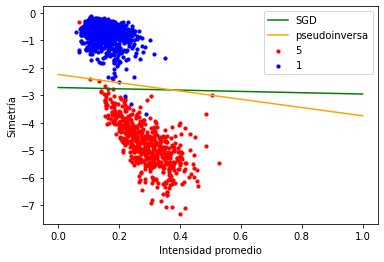
\includegraphics[width=\textwidth]{ej2.1_solucion_train}
		\caption{Train}
	\end{subfigure}
	\begin{subfigure}{0.5\textwidth}
		\centering
		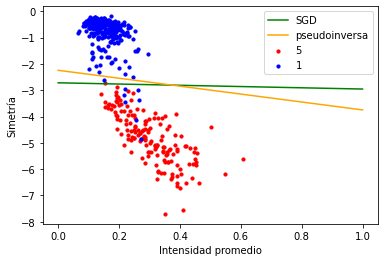
\includegraphics[width=\textwidth]{ej2.1_solucion_test}
		\caption{Test}
	\end{subfigure}
	\caption{Soluciones obtenidas en ambos algoritmos junto con los conjuntos de datos}
	\label{fig:ej2.1_soluciones}
\end{figure}

Se puede ver a simple vista que, tanto para los datos de entrenamiento como para los de test, ambos algoritmos obtienen rectas que separan con bastante acierto los elementos pertenecientes a distintas clases. Los errores obtenidos para cada algoritmo se pueden ver en el Cuadro \ref{fig:ej2.1_errores}. $E_{in}$ y $E_{out}$ son los errores devueltos por la función de pérdida para los conjunto de entrenamiento y test, respectivamente. $E_{in-clasif}$ y $E_{out-clasif}$ son los errores de clasificación, es decir, el porcentaje de elementos que han sido mal clasificados de los conjuntos de entrenamiento y test, respectivamente.

Podemos apreciar que el algoritmo de la pseudoinversa obtiene resultados ligeramente mejores que SGD, aunque esta diferencia es muy pequeña. En general, los dos algoritmo consiguen separar satisfactoriamente los elementos que pertenecen a diferentes clases, teniendo ambos en entrenamiento un error de clasificación inferior al 1 \% y, en test, inferior al 2 \%.

\begin{table}[]
	\centering
	\begin{tabular}{l|r|r|}
		\cline{2-3}
		& \multicolumn{1}{c|}{SGD} & \multicolumn{1}{c|}{Pseudoinversa} \\ \hline
		\multicolumn{1}{|l|}{$E_{in}$}         & 0.08165086935172927      & 0.07918658628900395                \\ \hline
		\multicolumn{1}{|l|}{$E_{out}$}        & 0.13486487694930924      & 0.13095383720052578                \\ \hline
		\multicolumn{1}{|l|}{$E_{in-clasif}$}  & 0.640615 \%              & 0.512492 \%                        \\ \hline
		\multicolumn{1}{|l|}{$E_{out-clasif}$} & 1.886792 \%              & 1.650943 \%                        \\ \hline
	\end{tabular}
	\caption{Tabla con los errores de la función de pérdida y de clasificación obtenido en SGD y en pseudoinversa}
	\label{fig:ej2.1_errores}
\end{table}



\subsection{Ajuste de modelos de regresión lineal con aumento de complejidad}

En este apartado, realizaremos un análisis de cómo cambian los errores $E_{in}$ y $E_{out}$ cuando aumentamos la complejidad del modelo lineal usado. Durante todo este apartado, el algoritmo que elegiremos para resolver el problema mediante regresión lineal será SGD. Primero, llevaremos a cabo un experimento en el que usaremos únicamente transformaciones lineales, tal y como hemos hecho anteriormente. Luego, repetiremos el experimento añadiendo transformaciones no lineales y compararemos los resultados obtenidos.

\subsubsection{Experimento con transformaciones lineales}

En primer lugar, generamos una muestra de entrenamiento pseudoaleatoria de $N = 1000$ en el cuadrado $X = [-1,1] \times [-1,1]$ mediante la función \codeword{simula_unif}. En la Figura \ref{fig:ej2.2_muestra} podemos ver la muestra obtenida.

\begin{figure}[h]
	\centering
	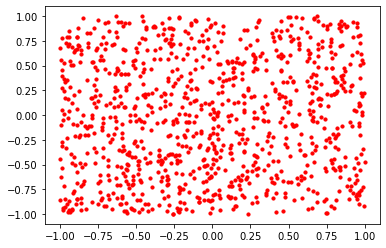
\includegraphics[width=0.6\textwidth]{ej2.2_muestra}
	\caption{Muestra de entrenamiento de $N = 1000$ en el cuadrado $X = [-1,1] \times [-1,1]$}
	\label{fig:ej2.2_muestra}
\end{figure}

A continuación, usando la función $f(x_1,x_2) = sign((x_1-0.2)^2 + x_2^2 - 0.6)$ etiquetamos la muestra. Los puntos que verifican la ecuación $(x_1-0.2)^2 + x_2^2 - 0.6 = 0$ forman una elipse, luego la función $f$ asigna un 1 a los puntos que están fuera de dicha elipse y un -1 a los que están dentro. Posteriormente, añadimos ruido cambiando el signo de las etiquetas con una probabilidad del 10 \%. La muestra etiquetada se puede ver en la Figura \ref{fig:ej2.2_muestra_etiquetada}.

\begin{figure}[h]
	\centering
	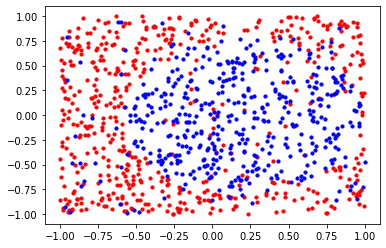
\includegraphics[width=0.6\textwidth]{ej2.2_muestra_etiquetada}
	\caption{Muestra de entrenamiento etiquetada con un 10 \% de ruido}
	\label{fig:ej2.2_muestra_etiquetada}
\end{figure}

A partir de la muestra creada, tomamos para cada punto el vector de características $(1,x_1,x_2)$ y usamos SGD para estimar los pesos $w$. Como hiperparámetros, fijamos $\eta = 0.05$, $batch\_size = 16$, $max\_epochs = 10$, 
$error = 0.001$ y $w_0 = (0,0,0)$. Después de ejecutarlo, obtenemos que $E_{in} = 0.9173293595181189$ y $E_{in\_clasif} = 37 \%$. En la Figura \ref{fig:ej2.2_sgd_lineal} podemos ver la recta ajustada sobre la nube de puntos etiquetada.

\begin{figure}[h]
	\centering
	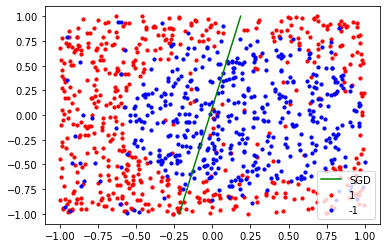
\includegraphics[width=0.6\textwidth]{ej2.2_sgd_lineal}
	\caption{Recta obtenida por SGD sobre la muestra etiquetada}
	\label{fig:ej2.2_sgd_lineal}
\end{figure}

Por último, para evitar que los sesgos asociados a la muestra con la que hemos estado trabajando hasta ahora influyan en la valoración posterior, repetimos todos estos pasos 1000 veces (generamos nuevas muestras de forma análoga con ayuda de la función \codeword{generateLabeledSample}). Además, para cada una de estas iteraciones, generamos una nueva muestra que usaremos para calcular el valor de $E_{out}$ y $E_{out\_clasif}$. Una vez ejecutadas todas ellas, calculamos los valores medios de cada uno de los errores, obteniendo lo siguiente:

\begin{itemize}
	\item Valor medio $E_{in}$: 0.930716239859433
	\item Valor medio $E_{in\_clasif}$: 39.9159 \%
	\item Valor medio $E_{out}$: 93.58520832673182
	\item Valor medio $E_{out\_clasif}$ Clasificación: 40.1056 \%
\end{itemize}


Se puede apreciar, tanto en los errores medios de clasificación (que se encuentran alrededor del 40 \%) como en la representación de la recta sobre la primera muestra tomada, que la solución obtenida no separa correctamente los puntos. La complejidad de la nube de puntos, los cuales podemos ver a simple vista que forman una elipse, no pueden ser clasificados de forma satisfactoria con una función tan simple como como una recta. Por tanto, es necesario hacer uso de una función de una mayor complejidad.



\subsubsection{Experimento con transformaciones no lineales}

Para este experimento, añadiremos términos cuadráticos al vector de características anterior, luego será de la forma $(1, x_1, x_2, x_1 x_2, x_1^2, x_2^2)$. Las muestras pseudoaleatorias seguirán siendo generadas de forma análoga a como lo hicimos anteriormente. También usaremos los mismos hiperparámetros de antes.

Empezamos tomando una muestra y ajustando una función mediante SGD a partir de los nuevos vectores de características. Los errores obtenidos son $E_{in} = 0.5621078673823251$ y $E_{in\_clasif} = 14.6 \%$. En la Figura \ref{fig:ej2.2_sgd_no_lineal} podemos ver la función ajustada sobre la nube de puntos.

\begin{figure}[h]
	\centering
	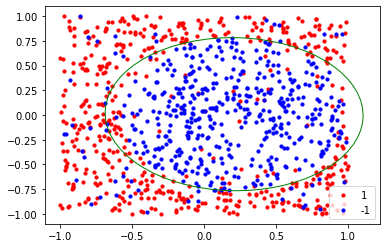
\includegraphics[width=0.6\textwidth]{ej2.2_sgd_no_lineal}
	\caption{Función no lineal obtenida por SGD sobre la muestra etiquetada}
	\label{fig:ej2.2_sgd_no_lineal}
\end{figure}

De nuevo, pero esta vez con vectores de características no lineales, ejecutamos SGD sobre 1000 muestras para las cuales obtenemos $E_{in}$ y $E_{in\_clasif}$. A continuación, generamos otras 1000 muestras para calcular $E_{out}$ y $E_{out\_clasif}$. Los valores medios obtenidos para cada uno de los errores son los siguientes:

\begin{itemize}
	\item Valor medio $E_{in}$: 0.5824299565059969
	\item Valor medio $E_{in\_clasif}$: 14.286700000000002 \%
	\item Valor medio $E_{out}$: 59.07117748965567
	\item Valor medio $E_{out\_clasif}$ Clasificación: 14.650099999999997 \%
\end{itemize}

Comparando los resultados obtenidos en ambos experimentos vemos que, al considerar transformaciones no lineales, los errores $E_{in}$ y $E_{out}$ se reducen casi a la mitad y los errores de clasificación pasan del 40 \% al 14 \% aproximadamente. Teniendo en cuenta que sería extraño que este último error tomase valores inferiores al 10 \% (pues es el porcentaje de puntos ruidosos que hemos introducido), considero que un 14 \% de error en clasificación es un resultado muy satisfactorio. Además, la Figura \ref{fig:ej2.2_sgd_no_lineal} apoya gráficamente la calidad de esta última solución, ya que la función obtenida (la cual es precisamente una elipse) encierra a la gran mayoría de puntos azules al mismo tiempo que muy pocos puntos rojos se quedan dentro de ella. Por todas estas razones, considero que el modelo con transformaciones no lineales obtiene resultados mucho mejores que el modelo que solo utiliza transformaciones lineales.







\newpage

\section{Bonus: Método de Newton}

El método de Newton es un algoritmo iterativo para encontrar aproximaciones de raíces de funciones. Si aplicamos este algoritmo sobre la primera derivada de la función (o su gradiente si la función es de varias variables), podemos encontrar máximos o mínimos de ésta. Esto último será lo que llevaremos a cabo para intentar llegar a un mínimo de la función $f$ definida en el primer ejercicio.

El método de Newton tiene un funcionamiento similar a gradiente descendente. Lo único que cambia es la regla de actualización del punto $w$, ya que ahora también usaremos la matriz hessiana. Esta matriz está formada por las derivadas de segundo orden de la función que se quiere minimizar. Por tanto, tenemos que calcular la matriz hessiana de la función $f$, que es la siguiente:

\begin{equation}
	\nabla^2 f(x) = 
	\left(
	\begin{matrix}
		2-8 \pi^2 \sin(2 \pi x) \sin(2 \pi y) & 8 \pi^2 \cos(2 \pi x) \cos(2 \pi y)\\
		8 \pi^2 \cos(2 \pi x) \cos(2 \pi y) & 4-8 \pi^2 \sin(2 \pi x) \sin(2 \pi y)
	\end{matrix}
	\right)
\end{equation}

La regla de actualización es: $w_{i+1} = w_i - \eta [\nabla^2 f(w_i)]^{-1} \nabla f(w_i)$.

Desarrollamos ahora los mismos experimentos que llevamos a cabo anteriormente para $f$. Fijamos $max\_iter = 50$ y $w_0 = (-1, 1)$ y ejecutamos el algoritmo para las tasas de aprendizaje $\eta = 0.01$ y $\eta = 0.1$. En la Figura \ref{fig:bonus_graficas} podemos ver las gráficas de $f$ junto con los mínimos obtenidos para cada una de las tasas de aprendizaje. Para $\eta = 0.01$ obtenemos el mínimo $(-0.9793498427941949, 0.9893767407575305)$, mientras que para $\eta = 0.1$ llegamos al mínimo $(-0.9463274028190676, 0.9717082373563009)$.

\begin{figure}[h]
	\begin{subfigure}{0.5\textwidth}
		\centering
		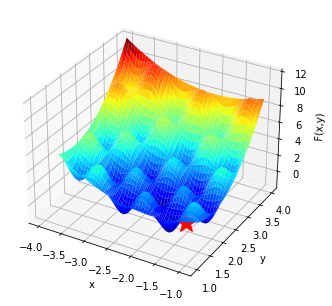
\includegraphics[width=\textwidth]{bonus_grafica_eta0.01}
		\caption{$\eta = 0.01$}
	\end{subfigure}
	\begin{subfigure}{0.5\textwidth}
		\centering
		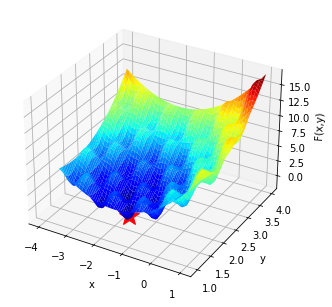
\includegraphics[width=\textwidth]{bonus_grafica_eta0.1}
		\caption{$\eta = 0.1$}
	\end{subfigure}
	\caption{Gráfica de $f(x,y)$ junto con el mínimo encontrado por el método de Newton}
	\label{fig:bonus_graficas}
\end{figure}

Por otro lado, si guardamos los valores que nos devuelve la función $f$ para cada uno de los mínimos $w$ obtenidos en cada iteración, podemos generar gráficas que muestren la evolución de dichos valores para ambas tasas de aprendizaje. En la Figura \ref{fig:bonus_evolucion} podemos ver esta evolución para $\eta = 0.01$ y $\eta = 0.1$, respectivamente.

\begin{figure}[h]
	\begin{subfigure}{0.5\textwidth}
		\centering
		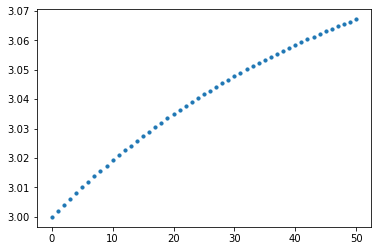
\includegraphics[width=\textwidth]{bonus_evolucion_eta0.01}
		\caption{$\eta = 0.01$}
	\end{subfigure}
	\begin{subfigure}{0.5\textwidth}
		\centering
		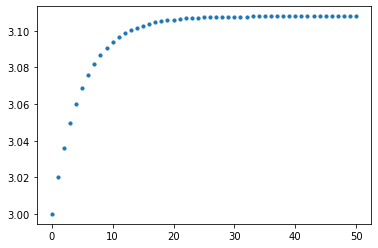
\includegraphics[width=\textwidth]{bonus_evolucion_eta0.1}
		\caption{$\eta = 0.1$}
	\end{subfigure}
	\caption{Evolución de los valores devueltos por los mínimos obtenidos en cada iteración}
	\label{fig:bonus_evolucion}
\end{figure}

Comprobamos que la evolución de ambas tasas de aprendizaje es creciente, devolviendo como resultado puntos que son peores a los iniciales. Aunque pueda parecer extraño, es algo que puede ocurrir, pues el método de Newton aplicado al gradiente de una función está diseñado para encontrar puntos críticos, es decir, puntos en los que el gradiente se anula. Estos puntos críticos pueden ser mínimos locales, máximos locales u otra clase de puntos.

También vemos que la evaluación en $f$ del punto final obtenido para $\eta  = 0.01$ es ligeramente inferior a la obtenida usando $\eta = 0.1$. Esto es debido precisamente a la tasa de aprendizaje, pues al ser menor, los cambios en el punto son menores y no consigue evolucionar tanto como el punto ejecutado con la tasa de aprendizaje mayor. 

Ahora, tomamos el mismo conjunto de puntos iniciales del primer ejercicio y ejecutamos el método de Newton con cada uno de ellos fijando $\eta = 0.01$. En el Cuadro \ref{fig:bonus_puntos_iniciales} podemos ver los resultados obtenidos. Si comparamos los valores mínimos obtenidos con gradiente descendente y con este método, vemos que este último obtiene resultados peores para todos los mínimos (excepto para el punto inicial $(-2.0, 2.0)$, el cual ya es mínimo local luego ambos algoritmos lo devuelven como mínimo).

\begin{table}[]
	\centering
	\begin{tabular}{|r|r|r|}
		\hline
		\multicolumn{1}{|c|}{\textbf{Punto inicial}} & \multicolumn{1}{c|}{\textbf{Mínimo}} & \multicolumn{1}{c|}{\textbf{Valor mínimo}}                          \\ \hline
		(-0.5, -0.5)                                 & (-0.44790207, -0.51725364)           & 15.012564277395944                                                   \\ \hline
		(1.5, 1.5)                                   & (1.51212294, 1.46428185)             & 12.875125450122088                                                   \\ \hline
		(2.1, -2.1)                                  & (2.11759899, -2.07774574)             & 49.57852918928263                                                  \\ \hline
		(-3.0, 3.0)                                  & (-3.02065016, 3.01062326)            & 3.067185951548828                                                \\ \hline
		(-2.0, 2.0)                                  & (-2.0, 2.0)                          & $-4.799231304517944 \cdot 10^{-31}$                                 \\ \hline
	\end{tabular}
	\caption{Tabla con los mínimos obtenidos para cada punto inicial}
	\label{fig:bonus_puntos_iniciales}
\end{table}

Podríamos extraer la conclusión de que el método de Newton es un algoritmo mucho peor que gradiente descendente. Sin embargo, el método de Newton aplicado al gradiente es un algoritmo que, como ya se ha dicho antes, no está preparado para encontrar mínimos sino puntos críticos. Y precisamente la función $f$ tiene muchos mínimos y máximos locales, además de otros puntos críticos que provocan que este método obtenga soluciones peores que los puntos iniciales de los que parte.


Con el objetivo de poner de manifiesto la potencia de este algoritmo cuando la función no es excesivamente complicada, decido aplicarlo sobre la función $E$ del primer ejercicio. Tomando una tasa de aprendizaje $\eta = 1$ y un punto inicial $w_0 = (1, 1)$, el método de Newton devuelve como mínimo el punto $(1.028 \dots, 0.617 \dots)$ en 7 iteraciones y cuyo valor mínimo es $3.0814879110195774 \cdot 10^{-33}$. Si comparamos con el primer ejercicio, tenemos que gradiente descendente, para el mismo punto inicial y $\eta = 0.1$, devolvía el mínimo $(1.157 \dots, 0.910 \dots)$ en 10 iteraciones y su valor mínimo era $3.1139605842768533 \cdot 10^{-15}$. La evolución de sus valores se puede ver en la Figura \ref{fig:bonus_evolucion_E}.

\begin{figure}[h]
	\begin{subfigure}{0.5\textwidth}
		\centering
		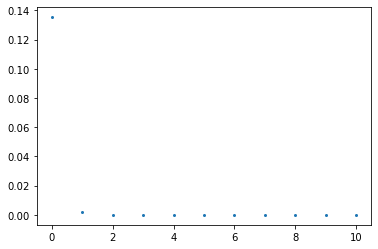
\includegraphics[width=\textwidth]{bonus_evolucion_E_gd}
		\caption{gradiente descendente}
	\end{subfigure}
	\begin{subfigure}{0.5\textwidth}
		\centering
		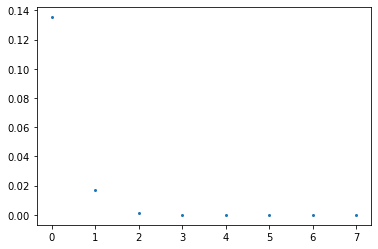
\includegraphics[width=\textwidth]{bonus_evolucion_E_newton}
		\caption{método de Newton}
	\end{subfigure}
	\caption{Evolución de los valores devueltos por los mínimos obtenidos en cada iteración}
	\label{fig:bonus_evolucion_E}
\end{figure}

Esto demuestra que el método de Newton es capaz de obtener resultados igual de buenos, o incluso mejores que gradiente descendente, eligiendo la tasa de aprendizaje adecuada, y siempre que la complejidad de la función no sea excesiva.




\end{document}



